\chapter{The importance of an architecture for autonomous systems}
\label{ch:prb}
\vspace{-1.3cm}

The development of an autonomous system is a process that involves various stages. Each stage is typically characterized by defining and solving issues related to different aspects of the system, ranging from the tasks it will be required to perform, to its construction and programming, and even to how the data it collects and that affect its operation should be presented to potential operators. Generalizing from a specific application case, most issues can be classified into a few high-level categories. Although it may seem counterintuitive from the division that follows, these categories are not always addressed sequentially, nor are they entirely independent of each other. To address situations like these, various project management techniques have been developed in recent times, aimed at minimizing the risk that an error made in an earlier phase could compromise subsequent stages, potentially undermining finished work and increasing development times. In light of the observations made in \Cref{ch:intro}, it is clear that, with the increasing complexity of modern automated systems and of the tasks they must perform, these topics are more relevant than ever. In particular, new tools made available to developers and designers will need to reflect these specificities, simplify the management of typical situations where possible, and highlight potential critical issues to aid in problem-solving. Practical experience shows that, despite the variety of cases and applications, the challenges faced are almost always, if not identical, very similar, as are the strategies to address them.

The aim of this chapter is to briefly present the issues typically encountered when designing an autonomous system, highlighting their unique characteristics without focusing on a particular application area, and then to examine some recent hardware and software solutions that enable the optimization of design, development, and testing activities. The discussion starts at a relatively high level of abstraction but becomes progressively more specific, forming the guiding thread that connects all subsequent chapters, finally highlighting the convenience of a well-structured software architecture to address the issues raised. The requirements that such an architecture must meet are then formalized and discussed in due detail.

Before moving further, it is instrumental to clarify the definition of an autonomous system in the context of this work. First of all, in this work the term \emph{system} identifies a macroscopic entity, which can either be entirely hardware, or entirely software, or a mixture of both, that evolves in time and is characterized by a set of inputs and outputs. Its tasks are defined by the operations that it must perform on these inputs to produce the desired outputs, and by the constraints that these operations must satisfy. The system can either be seen as a unitary entity or as a set of \emph{subsystems}, \emph{subcomponents}, and \emph{submodules}, all terms that are used interchangeably in this work, each of which takes care of a part of the processing, thus contributing to a part of the tasks. For the system to work correctly, all the subsystems must do the same and be interconnected accordingly, both in terms of the data they share and of the resources they use. The term \emph{autonomous} refers to the capability of the system to perform these tasks without human intervention, or with minimal human intervention, once it has been set up and started. This definition is intentionally broad and generic, as it is meant to encompass a wide range of applications and scenarios, \emph{e.g.}, from mobile robots to drones, from power plants to industrial automation systems. Another class of systems that is included in this definition and that is of interest in this work is that of \emph{dynamic systems}, which are systems whose state evolves in time according to a mathematical model that can be either deterministic or stochastic, and that can be either known or unknown. The evolution of the system's state, and thus that of its output, can be influenced by acting accordingly on its input, an operation that is commonly referred to as \emph{controlling} the system or \emph{applying a control law} to the system. In the context of autonomous systems this can be one of the tasks to perform, which is especially true for those systems that have a physical structure that can be modeled as a dynamic system and that should evolve over time according to a specific desired behavior.

\section{The design challenges of autonomous systems}
\label{sec:prb_design_challenges}
\subsection{Defining the tasks}
\label{sec:design_challenges_tasks}
The initial decisions in the design of an autonomous system concern the specifications of the operations that it performs. These specifications are fully defined from the onset down to the smallest detail possible at this stage, as they guide all subsequent choices, from hardware selection and construction to programming. During the breakdown of operational requirements into \emph{tasks}, intended as discrete units of work to be executed, various types emerge. Without delving, for now, into the specifics of a particular scenario, common categories of tasks include the following ones.

\begin{itemize}
    \item \textbf{Continuous tasks}, which begin at system startup and run uninterrupted until it is turned off or malfunctions.
    \item \textbf{Periodic tasks}, which are performed at regular intervals.
    \item \textbf{Asynchronous tasks}, which are executed only when a specific event occurs, which may or may not ever occur.
\end{itemize}

It is easy to see that most functionalities in modern autonomous systems can be broken down into tasks that fall within these categories. These include operations ranging from actuator control, to the collection of data and measurements required by control algorithms, to communication with operators and users. The system architecture should efficiently support the development of software modules and the integration of hardware solutions that can handle all these kinds of tasks.

\subsection{Choosing the hardware}
\label{sec:design_challenges_hardware}
The choices made initially in this direction may not be definitive, because they concern both the construction of the initial prototypes and the final product: there likely are misjudgments or unforeseen issues to address. Nevertheless, the hardware should be selected carefully based on the operational, structural, and construction requirements defined so far. Decisions taken in the previous step are of critical importance at this stage: establishing the computational complexity of the operations that the system has to perform dictates the kind of resources required from the hardware, which may need to be equipped with discrete coprocessors to handle specific types of data or subdivided into multiple interconnected subsystems. The term \emph{discrete} here refers to auxiliary hardware installed in a computer that cannot operate independently but is designed to be driven by the primary computer, providing specialized support for specific tasks.

A market survey is essential to assess whether pre-tested and ready-to-use components or SoCs (System-on-Chip) can be used rather than resorting to a proprietary solution, which generally entails significant development, testing, and certification costs. Another domain that adds its own level of complexity is that of lower-level hardware, which consists of:
\begin{itemize}
    \item high-speed \emph{microcontrollers};
    \item actuators;
    \item sensors;
    \item interfaces and communication devices;
    \item data storage systems.
\end{itemize}

Nothing more can be said about these elements without reference to a specific case. However, practical scenarios discussed later in this work follow this design practice. From the multiplicity of devices mentioned and that may compose a modern autonomous system, it starts to become clear how the complexity of the system can grow quickly, as anticipated in \Cref{ch:intro}. The need for a well-structured architecture becomes more evident.

\subsection{Organizing the software}
\label{sec:design_challenges_software}
Except for those components that perform crucial and highly specific functions, such as electrical or electronic circuits, nearly all operations carried out by a modern autonomous system are encoded within an internal computer, which translates these instructions into commands for other components. Given the underlying complexity of the system itself, the software that controls it also has a layered and highly hierarchical organization. In this hierarchy, the lower levels are occupied by modules that interact with the smaller and faster subsystems (\emph{e.g.}, the \emph{firmware}) and these modules are developed with particular attention to their characteristics and purposes. Moving up in the hierarchy, more modules are found that encode sophisticated operations such as supervision, planning, and user communication, making them closer to the notion of \emph{application} or \emph{system software}.

When operating in this context, it is essential to rely on tools that simplify design and development as much as possible at all levels, assisting with the management of issues related to module organization, inter- and intra-process communication, data processing, and storage of various data types. The convenience of a good architecture to handle these challenges becomes increasingly evident.

\subsection{Handling data}
\label{sec:design_challenges_data}
An autonomous system requires a nearly constant stream of information to complete its tasks. This information can be received in data packets managed by suitable communication interfaces, or it can be acquired directly through measurement devices commonly known as \emph{sensors}. For both solutions, typical challenges that arise immediately include the integration of these devices with the rest of the apparatus and the processing of the data they produce. These issues are crucial, as the operation of the entire system is almost always contingent upon obtaining information about measurable quantities of interest and the system's own state (consider, \emph{e.g.}, a feedback control algorithm).

It is therefore reasonable to expect that the hardware architecture of a modern autonomous system comprises numerous communication interfaces and sensors, the latter consisting of specific hardware designed to measure particular physical quantities of interest. The challenges mentioned above concern the integration of such hardware with the rest of the system and to the development of software modules capable of managing it, and of receiving and processing the data it generates.

\subsection{Debugging and testing}
\label{sec:design_challenges_testing}
As soon as the initial prototypes are finalized, testing should begin to verify functionality and confirm the validity of the design decisions that have been taken. Bearing in mind that a generic and universal testing procedure can not be defined, it can be expected that once hardware functionality is confirmed, attention shifts to software validation. Debugging software running on an autonomous system is in general more challenging than debugging common application software due to several specific factors, like the following ones.
\begin{itemize}
  \item It is more difficult to trace program execution on an autonomous, potentially mobile device: direct access to the system may not be available, and the tools at hand are often limited or not very sophisticated.
  \item In the event of issues, both the software and hardware in use must be checked as the problem may be due to hardware faults or incorrect use.
  \item Conducting tests is not as simple as running a program and verifying its results: the safety of the apparatus and its operators must be ensured throughout the entire procedure, which can make even the organization of a test a challenging task.
\end{itemize}

Given the difficulty and importance of this phase, it is reasonable to employ tools and methodologies that can facilitate these tasks as much as possible.

\section{Basic requirements}
\label{sec:prb_requirements}
The challenges outlined in the previous section are not exhaustive, nor are they entirely independent of each other. They are, however, representative of the issues that typically arise when designing an autonomous system. Summarizing briefly the many aspects previously covered, suppose that the task at hand is that of developing an autonomous system capable of performing a series of operations. It is reasonable, in the context of this work, to focus on situations that meet the following assumptions.
\begin{itemize}
  \item The system has a physical structure that can be modeled as a dynamic system, thus, one of the tasks consists in stabilizing and controlling this dynamic system, something that is commonly referred to in the following as \emph{low-level control} or simply \emph{control}.
  \item Digital programmable computers of different kinds are used to both develop and run all the algorithms, ranging from low-level control to task planning and supervision.
\end{itemize}
Note that the situations hereby described might span from mobile robots to drones and even power plants, all classes of systems that have been subject of this research work. Recalling \Cref{sec:prb_design_challenges}, a series of choices regarding the following items have to be made:
\begin{itemize}
  \item sensors and actuators to use;
  \item software tools and packages to employ and integrate;
  \item hardware platforms, \emph{i.e.}, onboard electronics to adopt.
\end{itemize}
Note how these items might be strongly interconnected. Low-level hardware has to be chosen according to the control objective for the underlying dynamic system, while high-level hardware is selected usually weighing the software that it runs against the physical capabilities, as well as the costs, of the system that is going to host it. Finally, software tools and packages can be divided in two groups: that which has to be developed from scratch, possibly very specific to the system at hand, and that which can be reused from existing libraries or frameworks. The latter category, for example, includes solutions for data processing, communication, and visualization, as well as remote access and monitoring tools; when one wants to develop the prototype of an autonomous system, especially for research purposes, these things may be overlooked but they are crucial for the system to be usable and maintainable and the overhead that they might introduce can easily become significant if not properly managed early on.

There is a principle in computer science \cite{raymond_how_2001}, dating back to the very early days of the discipline, stating that to do a proper job \emph{no problem should ever be solved twice} or, in a historical fashion, \emph{one must never reinvent the wheel} with the only exception of building a better wheel. One can see how this fits perfectly in the context of the development of autonomous systems: there is a wide range of complex foundational and integration problems to solve and present themselves each time a new system is developed. The scope of this work is to provide a solution that is \emph{reusable}, \emph{modular}, and \emph{maintainable} and that can be used as a foundation for the development of innovative prototypes and products. With this in mind, the following requirements are formally identified.
\begin{description}
  \item[(M) Modularity] The architecture should constitute both a development and deployment framework for solutions ranging from single modules, meant to be easily integrated and reused, to entire autonomous systems prototypes. To guarantee this, the structure of the framework should suit both these use cases: single modules should carry with them all their dependencies, and it should be possible to easily \emph{merge} single modules to build a \emph{superproject} out of many \emph{subprojects}.
  \item[(D) Development] The architecture should support the development of single modules both as standalone packages and as parts of the software suite of a prototype. While working on a superproject that integrates a module, it should be possible to modify and update the module easily propagating the updates to every other superproject which integrates that module, unless the superproject has been specifically configured to use a different version of the module. The architecture should also ease testing and debugging activities, independently of the environment in which a module is developed.
  \item[(A) Abstraction] The architecture should offer a \emph{system abstraction layer}, \emph{i.e.}, it should make it possible to carry on all the development activities without having to care too much about the underlying hardware on which a module or prototype software suite is deployed, apart from unavoidable specific differences, as well as to the target OS of such a platform. The architecture should ease deployment by offering a common framework across multiple different hardware platforms. In the end, the architecture shall offer very similar, if not equal, development and execution environments across different hardware platforms, requiring minimal effort to be replicated.
  \item[(O) Overhead] The architecture should be as lightweight as possible, in terms of both computational and storage resources. This is to ensure that the overhead introduced by the framework itself is minimal, and that the resources of the hardware platforms on which the framework is deployed can be used to their full potential for the tasks that the system is meant to perform.
\end{description}
Note that these requirements, if examined by the perspective of subjects such as systems engineering, might not appear well-posed due to, \emph{e.g.}, the lack of a clear and objective way to evaluate them. They are, instead, meant to guide the design of an architecture and not that of a specific system. Moreover, the design stage at which they are introduced is one in which many things still have to be evaluated such as, \emph{e.g.}, hardware platforms to support and preexisting software tools to integrate, and thus the final definition of the architecture is the result of many trade-offs. They are high-level requirements meant to guide the design process, characterizing the solution from a broad and functional point of view.

\section{Related work}
\label{sec:prb_related_work}
To further motivate the premises of this work, this section presents some of the most relevant solutions that have been proposed in recent years to address the issues outlined in \Cref{sec:prb_design_challenges}. The list, although short, is in fact exhaustive: to the best of the author's knowledge at the time of writing no other such framework has been developed and proposed in the literature. Furthermore, a review of the works presented hereafter would reveal to the interested reader that none of them fully meets the requirements identified in \Cref{sec:prb_requirements}, especially those that deal with the independence from the underlying hardware and the construction of a replicable development environment. Commercial and proprietary solutions have been voluntarily left out of this review: there exist commercial solutions that satisfy many requirements up to a certain point such as, \emph{e.g.}, MathWorks's MATLAB \cite{mathworks_matlab_nodate} and Simulink \cite{mathworks_simulink_nodate}. Such solutions, however, limit the capabilities of the user to what their vendors decide to provide, also imposing a mandatory organization to the user works. As the following chapters clarify, among the aims of this work there is also that of providing to users a platform that follows its own set of standards and practices, but at the same time does not enforce them in any way and does not require any proprietary tool, allowing instead the user to modify and expand any of its parts into what best suits their needs. Finally, to discuss the following, it is inevitable to mention solutions and tools which will be the subject of subsequent chapters: they will be presented in due detail in the following, while proper references are provided here. At the end of this section, a brief comparison of the solutions presented hereafter with respect to the requirements listed in \Cref{sec:prb_requirements} is provided in \Cref{tab:related_work}.

\subsection{RoboStack}
\label{sec:related_work_robostack}
The RoboStack framework \cite{fischer_robostack_2022}, published in 2022 and maintained ever since, constitutes a first promising solution to the challenges outlined in \Cref{sec:prb_design_challenges}. RoboStack is a collection of software packages built on the Conda package management system \cite{anaconda_inc_conda_nodate}, which has become the de-facto standard in both industry and academia for the management of Python \emph{environments}, a concept that has gained particular interest in the scientific community in recent years thanks to the popularity of Python as a programming language in contexts like big data processing, statistics, machine learning, and artificial intelligence. The Conda package manager allows to specify a set of software modules to be collected and installed in an isolated location, together with their specific versions in case such a level of granularity becomes necessary. Once such a configuration is specified, it can be replicated with ease on any other machine and filesystem path, regardless of the operating system and many other factors, thus providing a way to ensure that the software environment in which a program is developed and run is always the same. RoboStack builds on this concept, providing a wide set of software packages and libraries that are commonly used in the development of robotic systems, such as the Robot Operating System (ROS) and the Gazebo simulator, illustrated in \Cref{sec:ros2}, and that are sometimes difficult to install and configure correctly, especially on embedded platforms. The framework is designed to be used in conjunction with the Conda package manager, thus supporting a variety of operating systems ranging from Linux to Windows and macOS, and it is meant to be installed on machines that will be used for the development of robotic systems, deploying environments through the selection of specific sets of packages to install in each. This solution, although promising and already widely applicable, does not completely meet the requirements previously identified, for three reasons. First, it is entirely dependent on Conda which, although a very powerful tool, may not be the best choice in terms of \emph{isolation} of the software environment: while Conda allows one to install software packages in an isolated location, it does not provide a way to define a specific portion of system resources to offer to that software, a feature nowadays informally called \emph{containerization} and explained later on, which could be useful to further tune the performance of the software running on the system and ensure that the host OS installation stays intact. Second, every piece of software must be added to RoboStack to be installed in one of its environments, which means that the framework is not as flexible as it could be, as that it is not possible to install any software package available from any source out of the box; the addition process requires a variable amount of work, particularly due to the many dependencies a software module may have, as explained in \cite{fischer_robostack_2022}. Last, RoboStack is dependent on Jupyter for development, which is not the best choice in terms of development environments. While Jupyter is a very powerful tool, its main purpose remains that for which it has been originally developed: offering a way to write and run Python code multiple times in interactive notebooks displayed in a web browser, which is not really adherent to the scenario outlined at the beginning of this chapter which involves developing and testing in real time the software that will run on an autonomous system. Moreover, many plugins existing for other visualizers and IDEs, some of which are presented in the following sections, have to be reimplemented to be used in a Jupyter environment, which is not always possible or convenient. These limitations, although not critical, make RoboStack not the best choice for the development of autonomous systems, especially when the requirements identified in \Cref{sec:prb_requirements} are taken into account.

\subsection{eProsima Vulcanexus}
\label{sec:related_work_vulcanexus}
The Vulcanexus software suite \cite{eprosima_vulcanexus_nodate} developed by eProsima, originally released in early 2023, poses itself as a simple framework for the development of autonomous robotic systems. The suite is composed of a set of software packages that are meant to be installed either on a host operating system or inside a \emph{container} managed by, \emph{e.g.}, the Docker Engine presented in \Cref{sec:docker}. The suite is fairly lightweight but nonetheless comprehensive: it provides the Robot Operating System 2 (\ROS) middleware, together with the Fast DDS by eProsima \cite{eprosima_fast_nodate} implementation of the Data Distribution Service (DDS) communication middleware presented in \Cref{sec:dds}, plus some more software tools aimed at more specific scenarios like, \emph{e.g.}, that of microcontrollers. Moreover, the fact that it is shipped also as a Docker image, compatible with different hardware platforms, adds some flexibility to it in terms of isolation of both the development and execution environments with respect to, \emph{e.g.}, the aforementioned RoboStack framework. However, the major limitation of this framework lies in the fact that its features more or less end here. With respect to the requirements listed in \Cref{sec:prb_requirements}, no effort is made towards the construction of a modular development and deployment environment, nor towards the support to a wide range of hardware platforms, especially in the case of SoCs aimed at robotic systems which, as will be explained later on, are gaining an increasing interest by the scientific community but require a fair amount of effort to be correctly set up. Furthermore, the restriction to the Fast DDS communication middleware for \ROS, although evidently motivated by the fact that it is also developed by eProsima, hinders the flexibility of the framework in terms of communication protocols, an aspect that becomes critical in some operational scenarios where, \emph{e.g.}, the network is highly subject to packet loss as explained in \Cref{sec:zenoh}.

\subsection{EPICS}
\label{sec:related_work_epics}
EPICS (Experimental Physics and Industrial Control System) \cite{dalesio_epics_1991,epics_controls_epics_nodate} is a distributed software framework designed to meet the demanding requirements of control systems in experimental physics, particularly for large-scale accelerators and other complex installations. Originally developed at the Los Alamos National Laboratory, U.S.A., and first published in 1991, the aim of EPICS is to address the challenges of managing data acquisition, control processes, and supervisory management in high-performance environments, where existing industry solutions at the time were inadequate. EPICS is built on a distributed architecture that utilizes a software communication bus, allowing for the seamless integration of multiple functional subsystems. These subsystems include the Input/Output Controllers (IOCs), Display Manager, Alarm Manager, Archiver, and the Sequencer. Each subsystem is designed to operate in a distributed manner, ensuring that tasks can be easily distributed across nodes in a network, thereby scaling from small, localized test setups to expansive, highly distributed networks. The idea is that nodes in the network can represent either actual subsystems of the plant, or users connected to workstations that act as terminals, on which EPICS also run to let them and their software interact with the control system. The Channel Access protocol serves as the communication backbone of EPICS, providing a "software bus" for communication between various components of the system. Channel Access supports operations like connecting, getting, putting, and monitoring data fields across distributed databases, using both TCP and UDP protocols. This protocol enables subsystems, including user-extended components, to communicate efficiently. One of the core features of EPICS is its distributed database, which is hosted on IOCs and provides functionalities such as data acquisition, data conversion, alarm detection, and closed-loop control. The IOCs run on hardware platforms such as VME or VXI with a real-time vxWorks kernel and are connected via Ethernet. This configuration allows efficient execution of control tasks and the ability to extend the system easily by adding more controllers. Other main components share data to and from the database, in a distributed fashion. Among those there are multiple Managers, such as the Display Manager which provides a graphical interface to the current user connected to the workstation, and the Alarm Manager which keeps track of the state of all the alarms in the system and presents them in a hierarchical fashion to the rest of the architecture and to the users. EPICS also features a Sequencer, which uses a state notation language to manage the system through different operational states and handle exceptions. This sequencer allows for modal transitions of the IOCs, such as switching between operational modes or handling unexpected system events. EPICS has demonstrated considerable extensibility, allowing new hardware and software modules to be integrated with minimal modifications. This extensibility is further bolstered by ongoing upgrades to both hardware and software components to improve the system's performance and ease of configuration. Among the related frameworks considered in this context, EPICS is without any doubt the most relevant: it has been developed in a similar context to that of this work, \emph{i.e.}, that of physics research and development, and evolved into an industry-standard. However, its scale is also what makes it not applicable to the context of this work. EPICS is designed to manage large-scale installations, such as particle accelerators, and is not suitable for the development of small-scale prototypes or products, as it is too complex and resource-intensive, providing functionalities and services like, \emph{e.g.}, slow remote control and supervision. Moreover, its architecture is not modular, and it is not designed to be easily integrated with third-party software modules or libraries, which is a critical aspect in the context of this work. Finally, EPICS is not designed to be used on a wide range of hardware platforms, as it is tightly coupled with the vxWorks kernel and similar proprietary solutions which do not fit the practical contexts at which this work is originally aimed.

\subsection{BlockNet}
\label{sec:related_work_blocknet}
BlockNet \cite{calacci_blocknet_2020} is presented as a novel multiplatform control framework designed to address the limitations of existing control-oriented frameworks like, \emph{e.g.}, Simulink and EPICS. Unlike these alternatives, BlockNet aims to provide an integrated solution that supports simulations, real-time control, and the integration of complex technologies while maintaining execution order, ensuring dynamism, and achieving portability across different computing environments. The primary goal of BlockNet is to enable the seamless creation of local or distributed control systems by breaking down computations into individual code blocks that can be linked to form a computational network, completely similar to what would be the block diagram or Simulink diagram of a control system: the idea is exactly that of providing a framework for the development and deployment of control architectures starting from their modeling as block diagrams. This approach is highly beneficial in designing general-purpose control algorithms while maximizing code reusability. One of BlockNet's significant features is its capacity to execute these blocks in the correct order based on their input-output dependencies, thus ensuring deterministic behavior even in distributed systems. Moreover, BlockNet attempts to utilize all available computational resources by executing compatible blocks in parallel and incorporating asynchronous programming to improve overall efficiency. BlockNet is developed on top of the .NET framework, using the C\# language to ensure compiled-level portability across multiple operating systems and architectures, such as Windows, Linux, macOS, x86, ARM, and others. The use of .NET also enables effective memory management and provides support for modular extension of the framework, allowing users to add new functionality easily. BlockNet introduces communication primitives made available to nodes based on a \emph{publish-subscribe} paradigm, illustrated in \Cref{sec:dds}, but extends it to ensure deterministic execution, making it well-suited for real-time control applications. This paradigm allows easy distribution of data between blocks in a network or even across multiple machines without complex network configurations being required. BlockNet's distinguishing features include its emphasis on ease of use, dynamic adaptability, and extendibility. These characteristics make it suitable for a wide range of applications, from purely simulated environments to hardware-in-the-loop (HITL) systems. Unlike many existing frameworks, BlockNet allows the runtime modification of blocks and entire algorithms without the need for recompilation or system downtime, thereby enabling continuous integration and deployment scenarios in control engineering. The key architectural components of BlockNet range from timers and timing sources, to schedulers, data serializers, and mathematical libraries and solvers. BlockNet is indeed close to what could satisfy the requirements stated in \Cref{sec:prb_requirements}, although in that section lies also the main reason why it cannot be considered a solution to the problem that this work addresses. Apart from the fact that it starts from the aim of conceptually modeling distributed systems as block diagrams, a choice that may pose its own limitations, BlockNet tries to provide by itself a solution to any problem that, as the rest of this work illustrates, arises during the development of such a framework. This is a critical aspect, as it makes the framework less flexible and more complex than it could be, as well as prone to errors and design flaws, and less open to contributions from the scientific community. In contrast, this work starts from a thorough review of existing solutions that may solve parts of the original problem, requiring only some integration work and the development of what is missing; the next \Cref{ch:tools} is entirely devoted to the detailed description of such tools. Moreover, the choice of the .NET framework, although it is a very powerful and flexible tool, is not the best one in terms of portability and integration with third-party software modules and libraries, as it is a proprietary solution that is not widely used in the scientific community compared to other programming languages and toolchains, and that requires a specific development environment to be used as well as a certain degree of expertise to be developed with.

\subsection{NASA F Prime}
\label{sec:related_work_fprime}
The F Prime framework \cite{bocchino_f_2018}, developed in the United States by the Jet Propulsion Laboratory (JPL) of the National Aeronautics and Space Administration (NASA) and published in 2018, is currently one of the solutions that better fit the requirements listed in \Cref{sec:prb_requirements}. It is a lightweight, modular, and open-source framework for the development and deployment of software for small atmospheric and orbital vehicles like the CubeSats and the Mars Helicopter prototype. It provides the foundations for a software architecture oriented at flight control in which software modules, written in the C++ and Python programming languages, can be loaded and configured easily as \emph{components} of the architecture itself. The framework, due to its organization, encourages the development of software packages meant to be published and reused among subsequent missions and prototype developments. Moreover, the framework offers ad-hoc communication primitives and services, as well as some thread scheduling capabilities, to ensure that software tasks in the architecture meet their real-time requirements, an aspect that is crucial in flight and space operations. Finally, thanks to its light organization and basic system requirements, it supports a wide variety of general-purpose and real-time operating systems (RTOS) and can easily be compiled on many hardware architectures. This framework is very promising and shows a lot of potential, but still does not fully meet the aforementioned requirements, mainly because of its limited diffusion and specialized scope. Although it is open-source, it is aimed at a very specific scientific sector, that of space missions, thus receiving limited acclaim outside of such area. Moreover, a downside of its lightweight nature is that it offers limited support for the integration of third-party modules and libraries, a fact which limits the capability of the framework of being used in a wider range of scenarios comprising, \emph{e.g.}, that of swarm aerial robotics, as well as the potential benefit of contributions from the scientific community. Finally, as declared in \cite{bocchino_f_2018}, in its current version it depends on commercial, licensed software for some of its functionalities, which could be a limitation for users outside NASA and JPL.

\subsection{MARTe2}
\label{sec:related_work_marte2}
The MARTe2 framework \cite{fusion_for_energy_marte2_nodate}, standing for \emph{Multi-threaded Application Real-Time executor 2} \cite{neto_marte_2010}, is the second qualified framework that is presented in this section. Originally developed in 2005 by a team of nuclear fusion researchers at the Joint European Torus (JET) UK facility and then registered as a work of the Fusion For Energy (F4E) european organization, it has been under active development ever since and is currently employed in many nuclear fusion research facilities around the world. As its name suggests, it is a framework aimed at the development of real-time software control architectures, similar to the EPICS framework described in \Cref{sec:related_work_epics} but on a smaller scale. It is written in C++ and supports only this programming language. Its organization is actually the closest to what is requested in \Cref{sec:prb_requirements} and thus deserves a little deeper analysis. It is composed by a core set of libraries plus a set of optional "components" that add specific functionalities or support for particular hardware devices, algorithms, communication protocols, etc. As illustrated in \Cref{fig:marte2arch}, the core libraries are divided in three distinct groups:
\begin{itemize}
  \item \texttt{BareMetal}: a set of libraries that implement basic functionalities ranging from data types and hardware abstraction, to communication primitives and logging, and provide the definition of base classes that can be used to develop new components of an architecture.
  \item \texttt{FileSystem}: these libraries provide functionalities to read and write data from and to files, as well as to manage the configuration of the system and the logging of the data produced by the components.
  \item \texttt{Scheduler}: libraries in this group implement real-time thread schedulers and their algorithms, as well as models such as state machines that can be useful to keep track of the state of a software component or algorithm.
\end{itemize}
\begin{figure}[t!]
  \centering
  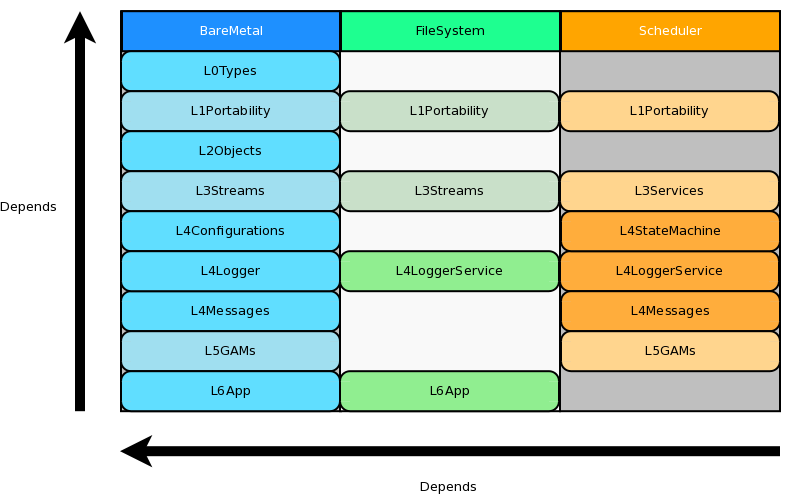
\includegraphics[width=.8\textwidth]{images/ch2/marte2_tiers.png}
  \caption{Organization of the core libraries of the MARTe2 framework \cite{fusion_for_energy_marte2_nodate}.}
  \label{fig:marte2arch}
\end{figure}
Moreover, note that libraries in each group follow a hierarchical organization, with those on the lower levels providing basic functionalities and those on the higher levels providing more complex and specialized ones. All of the framework and its components can be built using the GNU\footnote{GNU is Not Unix, \href{https://www.gnu.org/}{https://www.gnu.org/}.} \texttt{make} tool, as every MARTe2 software package comes with its own \texttt{Makefile} and the entire framework relies on a system of Makefiles that define environment variables and search paths for the compiler, then finally invoke it. The vision guiding the structure of the framework, although it has now reached a maturity that could make it applicable also in contexts that are completely different from nuclear fusion, \emph{e.g.} again, that of robotics, is still that of its early days: implement real-time software control architectures for physics research plants. Thus, its scope has remained the same ever since: managing software units that run \emph{algorithms} and exchange \emph{data} organized in \emph{signals}, which are collections of data of a specific type and dimension, modeling algebraic objects ranging from scalars to vectors and matrices. This idea reflects the main classes of software components that can be found and implemented in any MARTe2-based architecture, and that are the following:
\begin{itemize}
  \item \texttt{DataSource}: a component that exchanges data organized in signals with the external world, \emph{e.g.}, a hardware device or another software component.
  \item \texttt{Broker}: a component that manages the exchange of signals between higher-level components and \texttt{DataSources}, implementing memory synchronization schemes if required.
  \item \texttt{GAM}: short for \emph{Generic Application Module}, a component that implements an algorithm that processes input signals and produces output ones, \emph{e.g.}, a control algorithm or a data filtering algorithm.
\end{itemize}
Finally, a MARTe2-based architecture is usually divided in one or more applications, intended as processes running on the host machine, which contain a number of components specified in a configuration file together with their configuration parameters. Such configuration files, informally called \texttt{cfgs}, have a specific syntax, allowing an application to be built by literally "assembling" portions of a configuration file that define the components and their parameters, and then running the application with a specific configuration file that specifies the components to be loaded at run time, plus the settings for the OS scheduler. The reason why this work exists and MARTe2, although being the most promising solution, is still found in this section, is that as every other work hereby discussed it has its own downsides that set it a bit too much apart from the requirements stated earlier in this chapter. The first ones descend from its original scope, and recall the ones commonly found in previously examined works: it has been developed to aid in a very specific scientific research field, that of nuclear fusion in this case, and thus found very little to no adoption in the years outside of it; this translates to limited improvements over the original organization, and lack of support for modern technologies, third-party libraries, and use cases. The code organization and build system described early on is functional and efficient but follows old practices, like the focus on signals rather than software components, and relies on tools like \texttt{make} which, although standard and widely adopted, have nowadays been superseded by more modern solutions which are more suited to the management of large and modular codebases. Due to its strict real-time nature, MARTe2 also imposes some restrictions on the development of software modules, which must be written in C++ and must adhere to old language standards, lacking modern features and erecting a barrier against the integration of many open-source libraries and tools. These facts, together with the effective but cryptic syntax of the \texttt{cfgs}, make MARTe2 a very powerful but also clunky framework which often scares away newcomers and makes it difficult to maintain and evolve the software architectures built with it. Finally, although its compilation requires very little features from the host system, it is not officially supported on architectures other than \texttt{x86} and requires a tailored OS kernel to fully exploit its real-time capabilities, limiting its application in practice to Linux-based systems if one wants the smoothest possible usage experience.

\begin{table}[ht]
  \centering
  \begin{tabular}{|c|c|c|c|c|}
    \hline
    & \textbf{Modularity} & \textbf{Development} & \textbf{Abstraction} & \textbf{Overhead} \\
    \hline
    \textbf{RoboStack} & \checkmark & \xmark & \plusmark & \checkmark \\
    \hline
    \textbf{Vulcanexus} & \xmark & \plusmark & \plusmark & \checkmark \\
    \hline
    \textbf{EPICS} & \checkmark & \checkmark & \xmark & \checkmark \\
    \hline
    \textbf{BlockNet} & \checkmark & \plusmark & \plusmark & \xmark \\
    \hline
    \textbf{F Prime} & \checkmark & \plusmark & \plusmark & \checkmark \\
    \hline
    \textbf{MARTe2} & \checkmark & \plusmark & \plusmark & \checkmark \\
    \hline
    \textbf{DUA} & & & & \\
    \hline
  \end{tabular}
  \caption{Comparison of the solutions presented in \Cref{sec:prb_related_work} with respect to the requirements listed in \Cref{sec:prb_requirements}; ``\checkmark'' denotes a completely satisfied requirement, ``\plusmark'' indicates that the solutions provided do not fully satisfy a requirement, and ``\xmark'' marks an unsatisfied requirement. Is DUA, the framework presented later on in this work, going to meet them?}
  \label{tab:related_work}
\end{table}

